\PassOptionsToPackage{table,xcdraw}{xcolor}

%% For double-blind review submission, w/o CCS and ACM Reference (max submission space)
\documentclass[10p,conference]{IEEEtran}
\usepackage{times} 
\pagestyle{plain} % removes running headers

\bibliographystyle{IEEEtran}
%\citestyle{acmauthoryear}   %% For author/year citations
\usepackage{longtable}
\usepackage{url}
\usepackage{amsmath}
\usepackage{amsfonts}
\usepackage{amssymb}
\usepackage{listings}
\usepackage{color}
\usepackage{graphicx}
\usepackage{balance}

%% https://github.com/nickgian/thesis/blob/master/lstcoq.sty
\usepackage{color}

\definecolor{ltblue}{rgb}{0,0.4,0.4}
\definecolor{dkblue}{rgb}{0,0.1,0.6}
\definecolor{dkgreen}{rgb}{0,0.35,0}
\definecolor{dkviolet}{rgb}{0.3,0,0.5}
\definecolor{dkred}{rgb}{0.5,0,0}

% lstlisting coq style (inspired from a file of Assia Mahboubi)
%
\lstdefinelanguage{Coq}{ 
%
% Anything betweeen $ becomes LaTeX math mode
mathescape=true,
%
% Comments may or not include Latex commands
texcl=false, 
%
% Vernacular commands
morekeywords=[1]{Section, Module, End, Require, Import, Export,
  Variable, Variables, Parameter, Parameters, Axiom, Hypothesis,
  Hypotheses, Notation, Local, Tactic, Reserved, Scope, Open, Close,
  Bind, Delimit, Definition, Let, Ltac, Fixpoint, CoFixpoint, Add,
  Morphism, Relation, Implicit, Arguments, Unset, Contextual,
  Strict, Prenex, Implicits, Inductive, CoInductive, Record,
  Structure, Canonical, Coercion, Context, Class, Global, Instance,
  Program, Infix, Theorem, Lemma, Corollary, Proposition, Fact,
  Remark, Example, Proof, Goal, Save, Qed, Defined, Hint, Resolve,
  Rewrite, View, Search, Show, Print, Printing, All, Eval, Check,
  Projections, inside, outside, Def},
%
% Gallina
morekeywords=[2]{forall, exists, exists2, fun, fix, cofix, struct,
  match, with, end, as, in, return, let, if, is, then, else, for, of,
  nosimpl, when},
%
% Sorts
morekeywords=[3]{Type, Prop, Set, true, false, option},
%
% Various tactics, some are std Coq subsumed by ssr, for the manual purpose
morekeywords=[4]{pose, set, move, case, elim, apply, clear, hnf,
  intro, intros, generalize, rename, pattern, after, destruct,
  induction, using, refine, inversion, injection, rewrite, setoid_rewrite, congr,
  unlock, compute, ring, field, fourier, replace, setoid_replace, fold, unfold,
  change, cutrewrite, simpl, have, suff, wlog, suffices, without,
  loss, nat_norm, assert, cut, trivial, revert, bool_congr, nat_congr,
  symmetry, transitivity, auto, split, left, right, autorewrite},
%
% Terminators
morekeywords=[5]{by, done, exact, reflexivity, tauto, romega, omega,
  assumption, solve, contradiction, discriminate},
%
% Control
morekeywords=[6]{do, last, first, try, idtac, repeat},
%
% Comments delimiters, we do turn this off for the manual
morecomment=[s]{(*}{*)},
%
% Spaces are not displayed as a special character
showstringspaces=false,
%
% String delimiters
morestring=[b]",
morestring=[d]’,
%
% Size of tabulations
tabsize=3,
%
% Enables ASCII chars 128 to 255
extendedchars=false,
%
% Case sensitivity
sensitive=true,
%
% Automatic breaking of long lines
breaklines=false,
%
% Default style fors listings
basicstyle=\small,
%
% Position of captions is bottom
captionpos=b,
%
% flexible columns
basewidth={2em, 0.5em},
columns=flexible,
%
% Style for (listings') identifiers
identifierstyle={\ttfamily\color{black}},
% Style for declaration keywords
keywordstyle=[1]{\ttfamily\bfseries\color{dkviolet}},
% Style for gallina keywords
keywordstyle=[2]{\ttfamily\bfseries\color{dkgreen}},
% Style for sorts keywords
keywordstyle=[3]{\ttfamily\bfseries\color{ltblue}},
% Style for tactics keywords
keywordstyle=[4]{\ttfamily\color{dkblue}},
% Style for terminators keywords
keywordstyle=[5]{\ttfamily\color{dkred}},
%Style for iterators
%keywordstyle=[6]{\ttfamily\color{dkpink}},
% Style for strings
stringstyle=\ttfamily,
% Style for comments
commentstyle={\ttfamily\itshape\color{dkgreen}},
%
%moredelim=**[is][\ttfamily\color{red}]{/&}{&/},
literate=
    {fun}{{\color{dkgreen}{$\lambda\;$}}}1
    {bool}{{$\mathbb{B}$}}1
    {nat}{{$\mathbb{N}$}}1
    {Vforall2}{Vforall2}1 % quick workardoun to avoid partial replacement of 'forall' in identifier
    {nat\_equiv}{nat\_equiv}1 % quick workardoun to avoid partial replacement of 'nat' in identifier
    {forall}{{\color{dkgreen}{$\forall\;$}}}1
    {exists}{{$\exists\;$}}1
    {<-}{{$\leftarrow\;\;$}}1
    {=>}{{$\Rightarrow\;\;$}}1
    {==}{{\texttt{==}\;}}1
    {==>}{{$\Longrightarrow\;\;$}}1
%    {:>}{{\texttt{:>}\;}}1
    {->}{{$\rightarrow\;\;$}}1
    {<-->}{{$\longleftrightarrow\;\;$}}1
    {<->}{{$\leftrightarrow\;\;$}}1
    {<==}{{$\leq\;\;$}}1
    {\#}{{$^\star$}}1 
    {\\o}{{$\circ\;$}}1 
%    {\@}{{$\cdot$}}1 
    {\/\\}{{$\wedge\;$}}1
    {\\\/}{{$\vee\;$}}1
    {++}{{\texttt{++}}}1
    {~}{{\ }}1
    {¬}{{$\lnot$}}1     % this does not work
    {\@\@}{{$@$}}1
    {\\mapsto}{{$\mapsto\;$}}1
    {\\hline}{{\rule{\linewidth}{0.5pt}}}1
%
}[keywords,comments,strings]

\lstnewenvironment{coq}{\lstset{language=Coq}}{}

% pour inliner dans le texte
\def\coqe{\lstinline[language=Coq, basicstyle=\small]}
% pour inliner dans les tableaux / displaymath...
\def\coqes{\lstinline[language=Coq, basicstyle=\scriptsize]}

%%% Local Variables: 
%%% mode: latex
%%% Local IspellDict: british
%%% TeX-master: "main.tex"
%%% End: 
\usepackage{booktabs} 
\usepackage{subcaption}

\newcommand{\N}{\mathbb{N}}
\newcommand{\asnc}{\emph{ASN1C}}
 
\usepackage{amsmath}
\usepackage{amssymb}
\usepackage{latexsym}
\usepackage{relsize}
\usepackage{xcolor}
\usepackage{color}
\usepackage{mathtools}
\usepackage{enumitem}
\usepackage{multicol}

\usepackage{asn1}

%\usepackage{multicol}

\lstset{
  basicstyle=\ttfamily\small,
  frame=tb, % draw a frame at the top and bottom of the code block
  tabsize=4, % tab space width
  showstringspaces=false, % don't mark spaces in strings
  %numbers=left, % display line numbers on the left
  commentstyle=\color{green}, % comment color
  keywordstyle=\color{blue}, % keyword color
  stringstyle=\color{red}, % string color
  % identifierstyle=\color{grey},
}

\lstdefinelanguage{diff}{
    morecomment=[f][\color{diffstart}]{@@},
    morecomment=[f][\color{diffincl}]{+},
    morecomment=[f][\color{diffrem}]{-},
  }

\begin{document}

\title{Research Report: Formally-Verified ASN.1 Protocol C-language Stack}

\author{\IEEEauthorblockN{Nika Pona}

\IEEEauthorblockA{\textit{Digamma.ai}} \\ npona@digamma.ai

\and

\IEEEauthorblockN{Vadim~Zaliva}

\IEEEauthorblockA{Carnegie Mellon University\\Department of Electrical and Computer Engineering}\\vzaliva@cmu.edu

}


\maketitle

\begin{abstract}

    We describe our approach and progress in verification of a
  mature open-source ASN.1 compiler, \emph{ASN1C}, using the Coq proof
  assistant. Once completed, our project will provide state-of-the-art
  high assurance suitable for mission-critical systems. Furthermore, since
  formal verification will be layered atop a well-tested ASN.1
  stack, it will combine the benefits of high-performance portable
  stack implementation with formal correctness guarantees. As an essential step in our
  approach, the project will also provide a formalization of a key part of
  the ASN.1 standard. Such formal specification could subsequently be
  used by others to analyze ASN.1 properties and validate other
  implementations.

\end{abstract}

\section{Introduction}

\subsection{Background}

The ASN.1 (Abstract Syntax
Notation One) \cite{ASN1Intro} joint standard of the International
Telecommunication Union (ITU-T) and the International Organization for
Standardization (ISO/IEC) provides an essential interface description
language for defining data structures for serialization and
de-serialization in cross-platform data exchange.
 ASN.1 is vitally relied upon by core aspects of the
Internet infrastructure and Internet applications, such as telephony,
enterprise computing, utilities, finance, military, security,
digitally-controlled infrastructure, transportation, medical systems,
and commercial cloud computing.

Using ASN.1 language, one can define data structures that use
ASN.1 {\it primitive types}, such as \emph{INTEGER}, \emph{BOOLEAN}, \emph{OBJECT
IDENTIFIER}, and {\it constructed types}, such as \emph{SEQUENCE (OF)},
\emph{SET (OF)}, and \emph{CHOICE (OF)}. An example ASN.1 module that
describes an X.509-like public key certificate is shown in
Listing~\ref{lst:asnex} (revised for brevity). Such certificates, for example, are
used by every browser to access HTTPS web sites. The unabridged
version of the original ASN.1 definition for the X.509 standard takes
about 1,000 lines of ASN.1. 

\begin{lstlisting}[language=ASN1,label=lst:asnex,
  caption={ASN.1 example of X.509 certificates}]
X509 DEFINITIONS ::= BEGIN

  Certificate  ::=  SEQUENCE  {
    tbsCertificate       TBSCertificate,
    signatureAlgorithm   AlgorithmIdentifier,
    signature            BIT STRING
  }

  TBSCertificate  ::=  SEQUENCE  {
     version         [0]  INTEGER,
     serialNumber         INTEGER,
     signature            AlgorithmIdentifier,
     issuer               Name,
     subject              Name,
     subjectPublicKeyInfo SubjectPublicKeyInfo,
  }

  SubjectPubicKeyInfo ::= SEQUENCE {
    algorithm           AlgorithmIdentifier,
    subjectPublicKey    BIT STRING
  }

  AlgorithmIdentifier ::= SEQUENCE {
    algorithm           OBJECT IDENTIFIER
  }

  Name ::= SEQUENCE OF SET OF SEQUENCE {
    type                OBJECT IDENTIFIER,
    value               ANY DEFINED BY type
  }

END
\end{lstlisting}


A typical ASN.1 stack consists of a \textit{compiler} which parses
ASN.1 syntax definitions, as shown in the Listing~\ref{lst:asnex}, and
produces either a source code of a specialized protocol encoder/decoder for this data or a run-time data for a parametric protocol
encoder/decoder. 
  
\subsection{Motivation}

These days, embedded and user computing devices implement increasingly
vast numbers of essential functions and applications, many of which
exchange data using ASN.1. The ASN.1 standard is large and complex: it
currently comprises twelve sub-standards spanning 862 pages
supplemented by additional pages of corrigenda. This opens a door for
many potential software bugs and malicious exploits. As a result, the
interconnected communicating systems are becoming less stable and less
reliable, posing greater risks and potential dangers. Disruption of
the ASN.1 based communications could threaten the functioning of the
entire critical infrastructure our society relies upon.


The Computer Vulnerabilities and Exposures (CVE) database \cite{CVE}
lists critical ASN.1-related bugs that are found each year in the
existing systems. Noteworthy exposures have already been discovered
\cite{OpenSSLMemoryCorruption} that clearly illuminate potential vast
risk and exposure. We analyzed the last four years of ASN.1-related
issues reported in the CVE database\footnote{See Appendix~\ref{sec:vulnerabilities} for more
  details.}.  Among the vulnerabilities studied are CVEs for various
software and hardware products and vendors, including \textit{Apple},
\textit{axTLS}, \textit{Botan}, \textit{Bounty Castle},
\textit{librcrypto++}, \textit{libtasn}, \textit{LibTomCrypt},
\textit{Linux Kernel}, \textit{MatrixSSL}, \textit{Mozilla NSS
  (Firefox)}, \textit{Objective Systems}, \textit{OpenSSL},
\textit{PolarSSL}, \textit{RSA BSAFE}, \textit{Samba},
\textit{Samsung}, \textit{Snapdragon}, \textit{strongSwan}, and
\textit{Wireshark}.  Out of 52 problems analyzed, 39 are related to
memory safety, 6 related to stack and heap bounds checking, and 3 are
related to issues caused by applications accepting poorly formed ASN.1
input. Proving just following six formal properties can prevent 49 out of 52
vulnerabilities, which is more than 90\% of reported vulnerabilities:

\begin{enumerate}

\item Absence of read memory access violations (reading from memory locations outside of a permitted range).
\item Absence of write memory access violations (writing to memory locations outside of a permitted range).
\item Strict standard compliance (detecting not well-formed input)
\item Guaranteed parser program termination
\item Guaranteed bounds on stack size
\item Guaranteed bounds on heap size
\end{enumerate}

\subsection{Our approach}
\label{sec:approach}
To date, the relevant systems and methods are either (a) automatically tested but not
formally verified, (b) use verification approaches which rely on
automatic extraction from executable specifications (for example
involving network stack synthesis \cite{SEL4}, optimizing compilers
\cite{CompCert}, cryptographic libraries \cite{HACL}, and
encoder/decoders \cite{Narcissus}), or (c) apply a form of formal
verification which only proves partial correctness properties (partial
verification of NAT stack proving that only parts of DPDK are specification
compliant \cite{NAT}, partial verification of Linux kernel TCP
implementation with 55\% line coverage and 92\% protocol coverage
\cite{NSDI}). Consequently, (a) and (c) do not provide sufficient
correctness guarantees, while (b) is often impractical due to poor
performance and compatibility limitations. In contrast, we pursue a
far deeper and comprehensive verification approach to performance and
portability and seek to prove actual industrial-level C-code
implementation.

As shown in Figure~\ref{fig:components}, the project begins with ITU-T
standard document in the form of human-readable text. We manually
convert it into formal specification (H.spec). This is high-level
specification (in Coq) which describes the correspondence between data
types and packet octets data layout. This
specification is one of the outputs of this project and has a value of
its own.

\begin{figure}[h!]
  \centering
  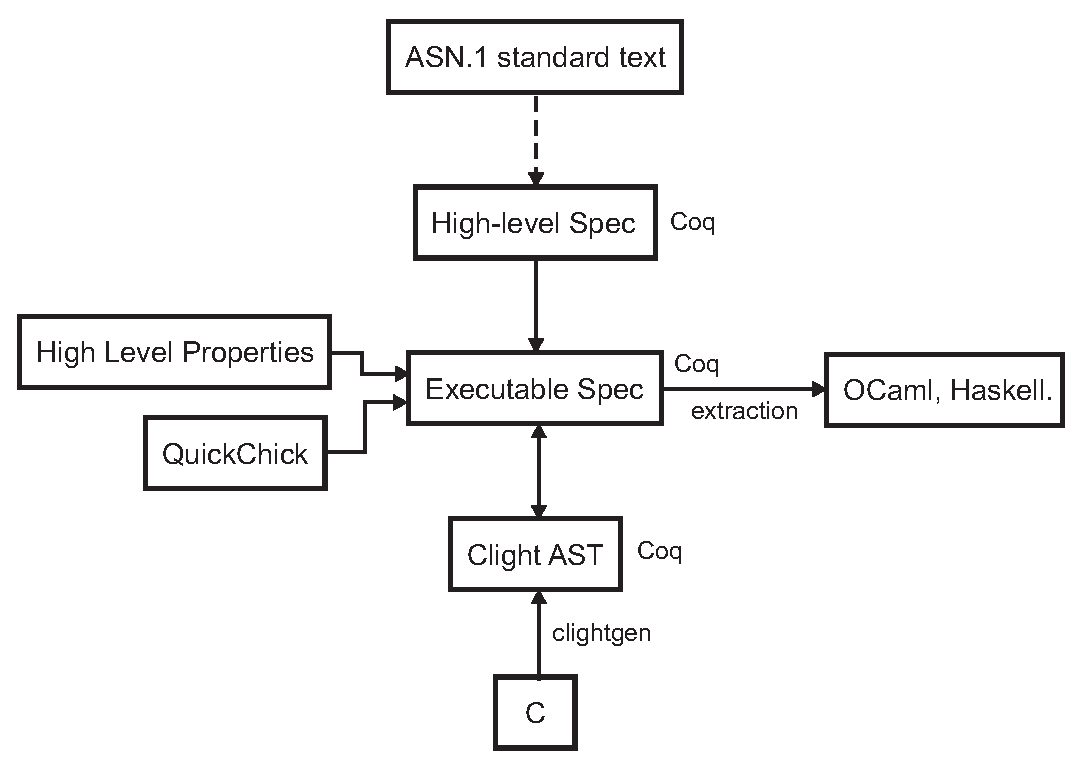
\includegraphics[width=9cm]{VerificationArchitectureDiagram.eps}
  \caption{Verification Architecture}
  \label{fig:components}
\end{figure}

The next level of refinement is executable specification (E.spec). Also
written in Coq, it declares ``encoder'' and ``decoder'' for each type
as a pair of pure functions and basically abstracts the encoding/decoding algorithm used in the C function and operates on abstract types such as Coq integers and lists of bytes. We prove that the E.spec encodes and decodes bytes in conformance with the high-level
specification. Moreover, we prove the roundtrip property for each encoder/decoder pair.

From E.spec we can \textit{extract} a fully functional encoder/decoder program in
languages supported by the Coq extraction mechanism (e.g. OCaml or
Haskell) \cite{Extraction}. Such a possibility is shown in the box
on the right in Figure~\ref{fig:components}, although we do not plan to
pursue it yet. However it could be explored in the future, for example,
in case we need to generate an ASN.1 stack for special platforms where
OCaml code opens some additional opportunities for parallelization,
optimization, or integration. One example of such platforms could be
MirageOS \cite{MirageOS}, which is an OCaml-based unikernel.

The box at the left, marked \textit{QuickChick}, represents another
possibility we might not pursue immediately. It uses randomized
property-based automated testing based on an executable
specification to further verify its correctness. This work could be
done using QuickChick \cite{QuickChick} in Coq. It could also be used
to generate a test-suite for the extracted code.

The next level is VST specification (VST.spec). VST stands for Verified Software Toolchain \cite{VST}, a tool that formalizes separation logic in Coq using operational C semantics from CompCert. It provides uniform syntax for stating pre- and postconditions of imperative programs execution, as well as tactics that automatize machine arithmetic and separation logic proofs. VST.spec states that the C program terminates and returns the machine representation of the value mandated by E.spec and that it satisfies the memory specification consisting of pre- and post-conditions written in separation logic. Correspondence to the memory specification guarantees memory safety. Further, we can add post-conditions about heap and stack bounds. 

At the bottom of Figure 1 is a box labeled ``C'' which represents the
existing C code of the \emph{ASN1C} compiler. Using an automated conversion
provided by the \texttt{clightgen} tool within the CompCert C compiler
\cite{CompCert}, we convert this to Abstract Syntax Trees (AST) (labeled ``C.AST'' in Figure 1) rendered from a subset
of C-language, called Clight \cite{Mechanized}, which is recognized by Coq. More specifically,
CompCert converts C ``concrete syntax'' to ``abstract'' Clight
syntax. The resulting Clight program is just a reification of the
original C program in Coq, retaining its overall structure; Clight is further assigned formal semantics
by CompCert that can be used to further reason about the behaviour of programs within Coq. 

Finally, as the most critical (and laborious) step of the project, we
prove that semantics of Clight
translation for each given function correspond to its VST specification. This guarantees that the C program terminates, is memory safe and behaves exactly like the executable and hence the high-level specification.



We perform all the proofs using the Coq Proof Assistant \cite{Coq}. From the
  proofs Coq can generate a ``certificate,'' which is a program in a
  formal language based on the Calculus of Inductive Constructions
  (``CIC'') \cite{CIC}. The certificate allows 3rd party
  validation of proofs which have been developed in Coq. The CIC is a small and mathematically
  well-defined formal language that serves as the underlying formal
  system of Coq. The generated certificate is automatically validated
  by the relatively small Coq kernel. Although a fraudulent
  certificate could hypothetically be created, it would not pass
  validation when submitted to the Coq kernel. The resulting outcome
  limits the trust need to rely only on the small CIC formal language and
  the small Coq kernel.

Additionally, our (modified) version of \emph{ASN1C} could be compiled with
the certified CompCert compiler \cite{CompCert} to extend correctness
guarantees through all levels down to machine code. This will provide state-of-the-art high
assurance suitable for mission-critical systems. Further, since formal
verification will be layered atop of a widely used ASN.1 stack, it
could be offered to current users immediately. This makes it attractive to new users who require higher
assurance levels than current non-verified implementations provide.

\section{Preliminary work}

Before committing ourselves to this project, we performed some initial
exploratory work to try different validation approaches, evaluate
tools and libraries, and estimate effort required. Briefly summarized
below are the results of some of the work we performed.

\subsection{Verifying floating-point numbers encoding}

As a first estimate of the difficulties associated with verifying
ASN.1-related programs, we wrote formal specification of an
encoder-decoder pair for a small but particularly error-prone subset
of the standard -- \textit{floating-point numbers}. The development is
available on github \cite{asn1fpcoq}. Our first approach was
relatively straightforward: define types representing ASN.1-encoded
data in Coq, provide functions for converting between representations,
and prove that they operate correctly. In particular, we proved the
roundtrip property for the defined encoders/decoders (i.e. the decoder is the inverse of the encoder).

Although providing guarantees of correctness, this technique has major disadvantages.
First of all, our definitions, being written in pure Coq, have only one
connection to the real world - through automatic code extraction.
This immediately creates a set of problems:

\begin{itemize}
\item Automatic code extraction from Coq is not formally verified.
\item Extracted code generally runs much slower than its counterparts implemented in other languages\footnote{The extracted code performed 15 times slower than the \emph{ASN1C}.}.
\item Extracted code might not be compatible with other code or viable in some real-world use-case scenarios.
\end{itemize}

However, this exploration allowed us to home in on what approaches
to verification are viable and improve our effort estimates. Moreover, we tested specification and proving techniques which will be useful for future experimentation.

\subsection{Verifying simple \emph{ASN1C} function}

To estimate the effort required to formally verify C code and to
experiment with various verification strategies, we decided to try to
verify a small function from an existing ASN.1 compiler. We chose
function \texttt{asn\_strtoimax\_lim} from the \emph{ASN1C} compiler. \emph{XER}
decoding functions for \emph{INTEGER}, \emph{OBJECT-IDENTIFIER}, and
\emph{RELATIVE-OID} types (and hence all constructed types that use
these primitive types) critically depend on this function. The
function is relatively simple but at the same time, it uses many features
of C that make verifying imperative programs challenging.

The only specification was the following comment in the source code:

\begin{quote}
 { \it Parse the number in the given string until the given *end position,
 returning the position after the last parsed character using the
 same (*end) pointer.
 WARNING: This behavior is different from the standard strtol/strtoimax(3). }
\end{quote}

Additional specification details must be inferred from the source code
and usage examples. Full source code of the function is included in
Appendix~\ref{sec:stritomax}.

\subsubsection{Problems discovered}

Despite that fact that this function lineage could be traced back 15
years and that it is part of mature, well-tested ASN.1 compiler presently used
in many production systems, we
found three bugs or problems in the current implementation. These had
never been reported before and had passed all human code reviews as
well as unit and fuzzying tests.
  
\paragraph{Negative range bug}

When we go beyond the allowed \textit{integer} range, an incorrect result is given
for some inputs. For example, assuming we are working on an 8-bit
system and the maximum signed integer (\texttt{MAX\_INT}) value is 127, parsing the input
string ``\texttt{-1281}'' is successful and returns the value -127 instead of the expected range error message. This happens whenever the input
string represents a number smaller than \texttt{MIN\_INT}, due to the
fact that its absolute value is greater than
\texttt{MAX\_INT}, thus the negative number cannot be treated as a
$\mathrm{value}\times\mathrm{sign}$ when the $\mathrm{value}$ is
represented as \textit{integer}. This bug was reported and promptly fixed by
developers.

\paragraph{Problem with pointer aliasing}

Another bug we discovered was related to potentially overlapping
memory areas pointed by argument pointers. Under some circumstances,
the value of the \texttt{end} pointer parameter is treated as a part
of the input data, and the resulting error value could be
incorrect. This bug would never occur if the function is always called
with non-overlapping pointer arguments. However this may be viewed
as an implicit pre-condition which should be part of the function's
specification.

\paragraph{Specification ambiguity}

After addressing the two bugs we discovered, we were able to
successfully verify that the function finally corresponds to the
specification we wrote for it. However, the following
behavior was noticed; for input ``\texttt{a}'', it records the value $0$ (the same behaviour
as for input ``\texttt{0}'') and returns the
\texttt{EXTRA\_DATA} error message (the same behaviour as for input
``\texttt{0a}''), which was probably unintended.
  
\subsubsection{Direct operational semantics proof}

First we formulated functional correctness and proved it using
big-step operational semantics of \textit{C light}, defined in
CompCert. In this proof, we used pure-function re-implementation in
Coq as an intermediate specification.

This function took addresses as inputs and operated on memory using
\texttt{load} and \texttt{store} operations from \textit{CompCert's}
memory model, while calculating the resulting machine integer
value. The proof went by induction on the distance between input
pointers and the main difficulty apart from trying to prove a faulty
program (that's when we discovered two bugs) was operational semantics
control flow minutiae and machine arithmetic proofs. However, only a
couple of lemmas about the specification were needed, and proofs of
different cases were very repetitive. Since functional and memory
specification were intertangled, it was more difficult to read the
specification and make sure it was correct. Hence, we missed the
specification ``bug'' mentioned above.

\subsubsection{Proof using VST}

The \textit{Verified Software Toolchain} offers solutions
to problems we encountered while doing direct operational semantics
proof; it has good automation of control flow, some automation for
machine arithmetic, and clear separation of functional and
memory-related parts of the specification. It also provides a uniform
way of stating functional correctness and memory safety, which reduces
the chances of having the wrong specification. Proofs here are done
using \textit{separation} logic implemented in Coq,
which are proven to be sound with respect to operational semantics of
CompCert. Similarly as before, we rely on C light syntax and
semantics. VST has tactics that can solve simple entailments in these
logics. However, they are not powerful enough to significantly reduce
the overall proof effort. In fact, with respect to memory safety
specifications, direct operational semantics proof were shorter and
more straightforward. However, this problem can be solved by improving
the existing tactics and fine-tuning the specification style, so in
the end we find this approach more viable for a large project.

In this simple example, we test our architecture from
Section~\ref{sec:approach}. First, we write a high-level specification
of this function in declarative, relational style (H.spec). Each constructor
corresponds to a return message (state) and stores a value and the
number of iterations of the function (used to store the result in
memory). Such specification can be easily examined and refined.

 \begin{lstlisting}[language=Coq]

(* Relation between input string, value, 
   index an asn_strtox_result_e error message *)
  Inductive asn_strtoimax_lim : list byte -> Z -> Z -> asn_strtox_result_e -> Prop :=
  (* Invalid data encountered *)
  | ERROR_INVAL:
      asn_strtoimax_lim nil 0 0 ERROR_INVAL
  (* More data expected (e.g. "+") *)
  | EXPECT_MORE : forall ls c,
      ls = [c]  ->
      is_sign c = true ->
      asn_strtoimax_lim ls 0 1 EXPECT_MORE
 (* Non-digit encountered *)
  | EXTRA_DATA : forall c ls z i,
      asn_strtoimax_lim ls z i OK ->
      is_digit c = false -> 
      asn_strtoimax_lim (ls ++ [c]) z i EXTRA_DATA
   ...    
  \end{lstlisting}

  The next level is the \textit{executable specification}
  \texttt{Z\_of\_string} (E.spec), which we prove to be equivalent to the
  relational specification. However, it could be extracted to Coq and
  is easier to use in future proofs of semantic equivalence with C
  code. Here, we experiment with two approaches. The function 
   \texttt{Z\_of\_string} can serve as a functional specification for
  \texttt{asn\_strtoimax\_lim} and differs little from the
  relational specification. 

 \begin{lstlisting}[language=Coq]
Fixpoint Z_of_string_loop (s : list byte) 
         (val i : Z) (b : bool) := 
    match s with 
    | [] => {| OK; val; i |}
    | c :: tl => 
      if is_digit c
      then let val' := app_char b val c in 
           if bounded val'
           then Z_of_string_loop tl val' (i + 1) b
           else {| ERROR_RANGE; val'; i; |}      
      else {| EXTRA_DATA; val; i; |}              
    end.

Definition app_char (b : bool) v c := 
  if b then v * 10 + (Z_of_char c) 
       else v * 10 - (Z_of_char c).
 \end{lstlisting}

 Since \texttt{Z\_of\_string} has a different structure from the C implementation, the proof requires many lemmas to
 connect functional specification to the C code and complicate the loop
 invariant. It is more effective to separate the
 functional aspect of the proof from the C-proof as much as possible to
 allow for more automation in the proof of C function
 correctness. Thus, we define another intermediate specification
 \texttt{Z\_of\_string\_C}, which is basically functional
 re-implementation of the C function, like the one used in the
 operational semantics proof but without mention of memory or machine integers. Then,
 we prove that \texttt{Z\_of\_string\_C} is equivalent to
 \texttt{Z\_of\_string}, which is a simple functional correctness
 proof that allows eliminating the need for additional lemmas in the
 C proof that connect the abstract specification with the C code structure.

 \begin{lstlisting}[language=Coq]
 
Fixpoint Z_of_string_loop_C (s : list byte)
          (val i : Z) (b : bool) := 
    match s with 
    | [] => {| OK; val; i |}
    | c :: tl => 
      if is_digit c
      then let d := (Z_of_char c) in 
           let val' := val*10 + d in
           if v <? upper_boundary 
           then Z_of_string_loop_C tl val' (i + 1) b
           else if (v =? upper_boundary)
                     &&(d <=? (last_digit_max b))
                then match tl with
                     | [] => {| OK; val'; (i + 1) |}
                     | c :: tl => 
                       if is_digit c
                       then {| ERROR_RANGE; 
                               app_char b val' c; 
                               (i + 1) |}
                       else {| EXTRA_DATA; 
                               val'; 
                               (i + 1) |}
                     end
                else {| ERROR_RANGE; val'; i |}      
      else {| EXTRA_DATA ; val; i |}              
    end.
    
 \end{lstlisting}

 We then wrote two VST specifications: one that uses the high-level specification
 and one that uses executable specification to state functional correctness. Memory specification for the function is expressed in terms of special memory or \emph{spatial}
 predicates. For instance, the predicate \texttt{(data\_at t ls p)}
 states that at the address \texttt{p} there is content \texttt{ls} of
 type \texttt{t}. One can combine such predicates with usual propositional connectives or with \emph{separation conjunction}
 (here written as \texttt{;}). Intuitively, if \texttt{P} and \texttt{Q} are spatial predicates, \texttt{p} and \texttt{q} are pointers, then  \texttt{(P(p) ; Q(q))} means that \texttt{P(p)} and \texttt{Q(q)} are true in separate sub-heaps of the memory or, in other words, that the pointers \texttt{p} and \texttt{q} don't overlap. Since we compare pointers between \texttt{str} and \texttt{*end} in the body of the function, we also have to ensure
 that they are valid pointers according to the C standard, are
 comparable (i.e. point within the same object), and non-overlapping. For instance, the
 memory precondition for the function will now have the following form:
\begin{lstlisting}[language=Coq]
PRE ((* str and *end are valid pointers *)
      valid_pointer *end; valid_pointer str ;
      (* str points to contents 
      ls of type char array  *)
      data_at (array char) ls str ; 
      (* end points to end' *)
      data_at (ptr char) *end end;
      (* intp points to some value v  *)
      data_at long v intp)
     \end{lstlisting}

     Moreover, the post-condition will record the changes in memory. We then
     prove that, given the precondition and after the execution of
     \texttt{asn\_strtoimax\_lim}, the post-condition will hold.
           
\begin{lstlisting}[language=Coq]
 POST((* the fist four lines of the precondition 
         didn't change after execution *)
      ... 
      let r := result (Z_of_string ls) in
       (* in 3 cases intp stays unchanged,
         otherwise store the end value
          of Z_of_string *)
       match r with 
         | ERROR_RANGE 
         | ERROR_INVAL 
         | EXPECT_MORE => 
           data_at long v intp
         | _ => data_at long 
                       (value (Z_of_string ls))
                        intp 
       end ;
      (* if str >= end, end doesn't change, 
         otherwise store the address of the last
          char read (before going out of range,
           reading extra data 
         or success) *)
       let i := index (Z_of_string ls) in
       if str <? *end
       then data_at (ptr char) (str + i) *end
       else data_at (ptr char) *end end).
\end{lstlisting}

Given experiments on this example, we delineated our strategy for proving
\emph{ASN1C} correctness as described in Section \ref{sec:approach}.

\section{Project Scope and Plan}

The International Telecommunications Union X.509 standard
\cite{X509} defines the format of public key certificates used in
many cryptographic Internet protocols (including TLS/SSL, the basis
for HTTPS protocol for secure browsing the web), certificate
revocation lists, certification path validation, electronic
signatures, and many other essential applications. X.509 is based on
ASN.1, using an important subset (Distinguished
Encoding Rules, ``DER'') of ASN.1 \cite{ASN1StandardBER} \cite{BERandDER}.

To limit the scope of the initial stage of the project while
exercising and showcasing all features of the complete ASN.1
standard, we focus the detailed verification on the DER part,
which can immediately be used to implement verified X.509
stacks for use in production applications.

The \emph{ASN1C} compiler supports BER, DER, CER, XER, PER and OER encoding/decoding rules. The total backend code is around 21,000 lines of code. We estimated X.509 related part to be around 3,000 lines of code. To compare, it took 18 person-years to write and verify 8,700 lines of code of \emph{sel4}, a formally verified operating-system kernel \cite{SEL4}. This gives us a conservative estimate of 6 person-years for this project. However, in the aforementioned project most of the time was used to develop technologies that are already available in the Coq community (formal semantics of C, some automation for machine integer arithmetic and separation logic proofs in VST). 

The X.509 focus provides a setting to answer after completion of the
1st stage essentially all questions
to determine the technical feasibility of the
proposed concept of full ASN.1 stack verification. These questions
include the following points:

\begin{enumerate}
\item How \emph{ASN1C} source code needs to be refactored to make it suitable for verification. In particular:
  \begin{enumerate}
  \item Which features of general C-language unsupported by CompCert's C language semantics need to be avoided?
  \item Are there any code organization changes which will aid structuring proofs (for example to make it easier to relate each function to a corresponding lemma)?
  \item Are there any simplifications which could be done to \emph{ASN1C} code by removing rarely used or obscure features that will make it easier to verify?
  \item Since the \emph{ASN1C} code base dates back more than a decade, are there are any low-level manual optimizations that could be eliminated by a combination of modern compilers and hardware that can handle them as well?
  \end{enumerate}
\item What high-level properties can be proven which will translate into additional code safety guarantees?
\item How should formalization of ASN.1 standard in Coq be written? - i.e. How to balance clarity, readability, and comprehensiveness?
\item How many of the proving steps could be automated and how can these automations speed up the proof process? Can they be used to estimate the effort required to prove the remainder of the ASN.1 stack?
\item How many of the proving methodologies and tools developed during the first phase could be re-used to prove similar software and other
  protocols?
  \item Are executable specifications of encoders/decoders completely sufficient to ``extract'' a working skeleton of the ASN.1 stack in OCaml? How much of additional ``glue'' code needs to be written to transform the result into a working product? How do code size and the performance of such extracted stack compare to the original C-language implementation from \emph{ASN1C}?  
\end{enumerate}

To address these questions determining the technical feasibility of
our proposed concept, we defined key tasks and objectives:

%The following key tasks are planned:
 
\begin{description}

\item[Task 1] Formalization of X.509-Relevant Parts of ASN.1 Specification

\item[Task 2] Refactoring of the ASN1C C Code Implementation of ASN.1

\item[Task 3] Primitive and Constructed Type Verification

\item[Task 4] Proof of Additional High-Level Properties 

\item[Task 5] Code Extraction from Execution Specification

\item[Task 6] Final Code, Associated Documentation, Estimates of Additional Work
 \end{description}


\section{Project Status}

Now, we are working in parallel on the high-level specification of the standard and executable specification of the \emph{ASN1C} encoders/decoders,  while recording changes that should be made to the C code.

 We start by formalizing BER and DER encoding rules for several primitive and constructed types in relational style. Each premise of a constructor formalizes (part of) a paragraph in the standard. E.g., for boolean type:

\begin{lstlisting}[language=Coq]
Inductive DER_Bool : bool -> list byte -> Prop :=
| False_Bool_DER : (* 8.2.2 *)
    DER_Bool false [all_zero]
| True_Bool_DER : (* 11.1 *)
    DER_Bool true [all_one].
\end{lstlisting}

Then we use our primitive type specifications to formalize DER relation for each type using predicates about length and tags. The formalization is first-order, thus it can be easily translated to other languages than Coq. Moreover, the relation to the text is straightforward, which will ease its inspection and validation.

\begin{lstlisting}[language=Coq]
Inductive DER : asn_value -> list byte -> Prop :=
| Bool_DER b t v:
    PrimitiveTag t ->  (* 8.2.1 *)
    DER_Bool b v ->
    DER (BOOLEAN b) (t ++ [Byte.one] ++ v)
      
| Integer_short_DER t v z : 
    PrimitiveTag t -> (* 8.3.1 *)
    length v = 1 ->   (* 8.3.2, case 1 *)  
    DER_Integer z v ->
    DER (INTEGER z) (t ++ [Byte.one] ++ v) 

| Integer_long_DER t l v z:
    PrimitiveTag t -> (* 8.3.1 *)         
    DefiniteLength (length v) l -> (* 10.1 *)
    1 < length v -> (* 8.3.2, case 2 *)
    v[1] != all_one ->  (* 8.3.2, (a) *)
    get_bit 7 v[1] = 1 -> (* 8.3.2, (b) *)
    DER_Integer z v ->
    DER (INTEGER z) (t ++ l ++ v) 
    ...

\end{lstlisting}

We write executable specification that is close to the actual implementation, since we have to keep in mind the future proof effort, especially with respect to
the C code. This involves devising structures and functions that are easily translatable to their C counterparts. 


The \emph{ASN1C} compiler has a modular structure, so we can proceed with
verification in a modular way by exploiting this structure. From a high-level view, the \emph{ASN1C} compiler consists of
the library of primitive type decoders (\emph{INTEGER}, \emph{BOOLEAN},
\emph{FLOATING POINT}, etc.). Each of these can be verified with respect to its
ASN.1 specification. Our previous work on floating point numbers is an example
of this. We start with the simplest types; we write the executable specification that corresponds to the C function; and then check it with respect to the specification. Even for the simplest boolean type, we find that the decoder was not behaving according to the standard; in particular, several encodings for boolean values were possible, which clearly violates the ASN.1 standard for DER encoding/decoding.


Furthermore, the compiler contains functions that decode/encode
constructed types (such as \emph{SEQUENCE}, \emph{CHOICE}, \emph{SET}). Then, from a
given ASN.1 type definition, the \emph{ASN1C} compiler produces an internal
representation of that type, specifying which existing
decoders/encoders to apply and in which order, as well as the
output/input C structures for the functions. In Coq,
these internal representations correspond to trees with nodes labelled by the
type's tags and decoder/encoder types.


 \begin{lstlisting}[language=Coq]
Inductive decoder_type := BOOLEAN | INTEGER ...

Inductive TYPE_descriptor :=
  DEF { tags : list Z;
        decoder : decoder_type;
        elements : list TYPE_descriptor 
      }.
 \end{lstlisting}

 Then, a constructed type decoder has type
 \lstinline[language=Coq]{TYPE_descriptor -> list byte -> option asn_value} and traverses the tree and applies the respective
 primitive decoders (this is a simplified definition; in the actual implementation, we use stream monad for input and monadic error handling).
 In \emph{ASN1C}, the decoder is implemented as a recursive
 function that readily translates into a nested or mutually recursive
 function in Coq.

 Given a particular ASN.1 type definition that translates into a
 \texttt{TYPE\_descriptor}, the \texttt{decoder} function for that
 particular type corresponds to a transition system with states where
 primitive decoders are called. Hence, one of the ways we can
 formalize the compiler is as a function that creates a transition
 system from a given ASN.1 type definition or \texttt{TYPE\_descriptor} tree. Since the run of the
 recursive \texttt{decoder} function corresponds to the transition
 system, we can use this model in the proof of implementation
 correctness.

 The \texttt{decoder} function could also be viewed in terms
 of a sequence parser combinator, known from the monadic parser combinators
 approach \cite{MPC}. Given decoders \lstinline[language=Coq]{p1, p2 : decoder asn_value} for primitive functions, it is possible to add an operator \lstinline[language=Coq]{seq} that takes two
 decoders and applies them sequentially \lstinline[language=Coq]{seq p1 p2}. Then the compiler can be seen as producing the
 concrete combination of parsers given the \texttt{TYPE\_descriptor}. Currently, we are experimenting with these approaches.

\balance

\section{Related Work}

Microsoft's EverParse project \cite{RamananandroDFS19} is the closest
to what we do. However, they don't verify the existing protocol stack but
build their own. They define their own input language which accepts
C-like type definitions, which automatically generate specifications, their implementations, and proofs of correctness. This is possible because the produced decoders are combinations of existing parsers that are proved correct in F*. They
follow the tradition of parser combinators. Starting with
  primitive parser combinators \texttt{fail}, \texttt{return[x]}, \texttt{read\_byte}, and monadic composition of
  two parsers \texttt{and\_then}, one can define combinators for
  parsing of pairs, mapping of functions on parser results, filtering of parser results etc. For each
combinator there are two implementations: functional and
C-like. C-like implementation is written in a subset of F* that models
imperative language, called Low*. Functions written in Low* operate on
memory addresses and use machine integer formalization. They rely on
automatic extraction from Low* to C using the tool Kremlin.

The project Narcissus \cite{Narcissus} also constructs correct binary parsers from a verified
library of combinators written in Coq, but it generates only functional
parsers and has the same disadvantages as our preliminary work on floating-point parsing. Built on Narcissus, there is a verified compiler in Coq for
parsers and formatters specified by Protocol Buffers.
 
Galois, Inc. did some work on ASN.1 verification in the past (circa
2012) \cite{ASN1FormalSem}. It appears that they abandoned the goal of
full ASN.1 verification \cite{ASN1EncDec} that we pursue in our
project with our more pragmatic approach; Galois is now only exploring
a limited subset ASN.1 verification adequate for the
``vehicle-to-vehicle'' (V2V) market \cite{V2V}, but that particular
subset has limited applicability, and their effort is limited by
constraints of their chosen approach.

The project is in active development right now, but given the
ambitious scope a significant effort is required for it's completion.
While Digamma.ai is committed to sponsor the initial stage of the
project, we are currently looking for industry and academic partners
to join us in the full ASN.1 verification endeavor.

\onecolumn
\appendix
\section{Appendix}

\subsection{\emph{asn\_strtoimax\_lim} source}

\label{sec:stritomax}

\lstinputlisting[language=C,basicstyle=\ttfamily\small]{asn_strtoimax_lim_old.c}

 \onecolumn
\subsection{ASN.1 Vulnerabilities Analysis}

\label{sec:vulnerabilities}

\scriptsize
\begin{longtable}{ l l l p{26em} }
 
  {\bf CVE } &  {\bf Product  } &  {\bf Property violated  }  &  {\bf Description  } \\

  \hline

2015-7061    & Apple *OS     & Memory safety (write) & remote attackers to execute arbitrary code or cause a denial of service (memory corruption) via a crafted certificate \\  
2015-7060    & Apple *OS     & Memory safety (write) & denial of service (memory corruption) via a crafted certificate \\  
2015-7059    & Apple *OS     & Memory safety (write) & denial of service (memory corruption) via a crafted certificate \\  
2018-16253   & axTLS         & Parsing only well-formed input & X.509 metadata verification \\ 
2018-16149   & axTLS         & Memory safety (read) & blindly trusts the declared lengths in the ASN.1 structure \\ 
2017-1000416 & axTLS         &  & coding error in the ASN.1 parser \\ 
2016-9132    & Botan         & Memory safety (write) & decoding BER data an integer overflow; memory corruption \\ 
2015-5726    & Botan         & Memory safety (read) & remote attackers to cause a denial of service (application crash) \\ 
2016-1000342 & Bouncy Castle & Parsing only well-formed input & introduction of 'invisible' data into a signed structure \\ 
2016-1000338 & Bouncy Castle & Parsing only well-formed input & introduction of 'invisible' data into a signed structure \\ 
2017-11496   & Gemalto ACC   & Memory safety (write) & remote attackers to execute arbitrary code \\ 
2016-9939    & libcrypto++   & Bounds on heap size & If there is not enough content octets in the ASN.1 object, then the function will fail and the memory block will be zeroed even if its unused. There is a noticeable delay during the wipe for a large allocation \\ 
2015-2806    & libtasn1      & Memory safety (write) & remote attackers to have unspecified impact via unknown vectors \\
2016-6129    & LibTomCrypt   & Memory safety (read) & does not validate that the message length is equal to the ASN.1 encoded data length \\
2019-9162    & Linux Kernel  & Memory safety (read/write) & out-of-bounds read and write operations possible \\
2016-2053    & Linux Kernel  & Parsing only well-formed input & Skipping non-optional fields after optional \\ 
2016-0758    & Linux Kernel  & Memory safety (read) & local users to gain privileges via crafted ASN.1 data \\ 
2019-13470   & MatrixSSL     & Memory safety (read) & out-of-bounds read \\ 
2016-6891    & MatrixSSL     & Memory safety (read) & (out-of-bounds read) via a crafted ASN.1 Bit Field primitive \\ 
2016-1950    & Mozilla NSS   & Memory safety (write) & remote attackers to execute arbitrary code via crafted ASN.1 data in an X.509 certificate \\ 
2015-7182    & Mozilla NSS   & Memory safety (write) & denial of service (application crash) or possibly execute arbitrary code \\ 
2015-7181    & Mozilla NSS   & Memory safety (write) & improperly restricts access to an unspecified data structure, which allows remote attackers to cause a denial of service (application crash) or possibly execute arbitrary code \\ 
2016-5080    & Objective Systems ASN1C & Memory safety (write) & execute arbitrary code or cause a denial of service \\ 
2018-0739    & OpenSSL       & Bounds on stack size & exceed the stack given malicious input with excessive recursion \\ 
2016-7053    & OpenSSL       & Memory safety (read) & crash with a NULL pointer dereference \\ 
2016-2842    & OpenSSL       & Memory safety (write) & remote attackers to cause a denial of service (out-of-bounds write or memory consumption) \\ 
 
2016-2176    & OpenSSL       & Memory safety (read) & remote attackers to obtain sensitive information from process stack memory or cause a denial of service (buffer over-read) \\ 
2016-2109    & OpenSSL       & Bounds on heap size & denial of service (memory consumption) \\ 
2016-2108    & OpenSSL       & Memory safety (write) & (buffer underflow and memory corruption) \\ 
2016-0799    & OpenSSL       & Memory safety (read/write) & remote attackers to cause a denial of service (overflow and out-of-bounds read) \\ 
2015-3195    & OpenSSL       & Memory safety (read) & obtain sensitive information from process memory by triggering a decoding failure in a PKCS\#7 \\ 
2015-3194    & OpenSSL       & Memory safety (read) & denial of service (NULL pointer dereference and application crash) via an RSA PSS ASN.1 signature \\ 
2015-1790    & OpenSSL       & Memory safety (read) & remote attackers to cause a denial of service (NULL pointer dereference and application crash) \\ 
2015-0289    & OpenSSL       & Memory safety (read) & attackers to cause a denial of service (NULL pointer dereference and application crash) \\ 
2015-0287    & OpenSSL       & Memory safety (write) & denial of service (invalid write operation and memory corruption) \\ 
2015-0286    & OpenSSL       & Memory safety (read) & denial of service (invalid read operation and application crash) \\ 
2015-0208    & OpenSSL       & & denial of service (NULL pointer dereference and application crash) \\ 
2015-1182    & PolarSSL      & Memory safety (write) & remote attackers to cause a denial of service (crash) or possibly execute arbitrary code \\ 
2018-11058   & RSA BSAFE     & Memory safety (read) & Buffer Over-Read vulnerability when parsing ASN.1 data \\ 
2018-11056   & RSA BSAFE     & Bounds on stack size & remote attacker could use maliciously constructed ASN.1 data that would exhaust the stack \\ 
2018-11054   & RSA BSAFE     & Native integer overflows & integer overflow vulnerability \\ 
2015-7540    & Samba         & Bounds on heap size & remote attackers to cause a denial of service (memory consumption and daemon crash) \\ 
2019-6740    & Samsung S9    & Memory safety (write) & does not properly validate the length of user-supplied data prior to copying it to a fixed-length heap-based buffer \\ 
2017-18315   & Snapdragon SOC & Memory safety (read) & Buffer over-read vulnerabilities \\ 
2017-9023    & strongSwan    & Termination & infinite loop in CHOICE parsing \\ 
2019-9209    & Wireshark     & Memory safety (write) & buffer overflow associated with excessive digits in time values \\ 
2019-5718    & Wireshark     & Memory safety (read) & boundary check to make sure we don't go past the end of "ptr" \\ 
2019-13619   & Wireshark     & Memory safety (read) & properly restricting buffer increments \\ 
2018-14343   & Wireshark     &  & integer overflow in BER lengths \\ 
2016-4421    & Wireshark     & Bounds on stack size & remote attackers to cause a denial of service (deep recursion, stack consumption, and application crash) via a packet that specifies deeply nested data \\ 
2016-4418    & Wireshark     & Memory safety (read) & remote attackers to cause a denial of service (buffer over-read and application crash) \\ 
2016-2522    & Wireshark     & Memory safety (read) & remote attackers to cause a denial of service (out-of-bounds read and application crash) \\ 
​\end{longtable} 


\begin{multicols}{2}\bibliography{report}\end{multicols}
\end{document}
